% !TEX root = ../main.tex
\documentclass[../main.tex]{subfiles}
\begin{document}

\section{Mathematical description of the poly-line separation measure}
\label{appendix:clustering_maths}

This appendix details the metric used in Section \ref{sec:aggregation_of_volunteer_models} to cluster poly\-lines used by volunteers to model spirals arms. It can be seen as a variant of the Fréchet distance. The metric is illustrated in Figure \ref{fig:spiral_metric_description}.

\begin{figure}
  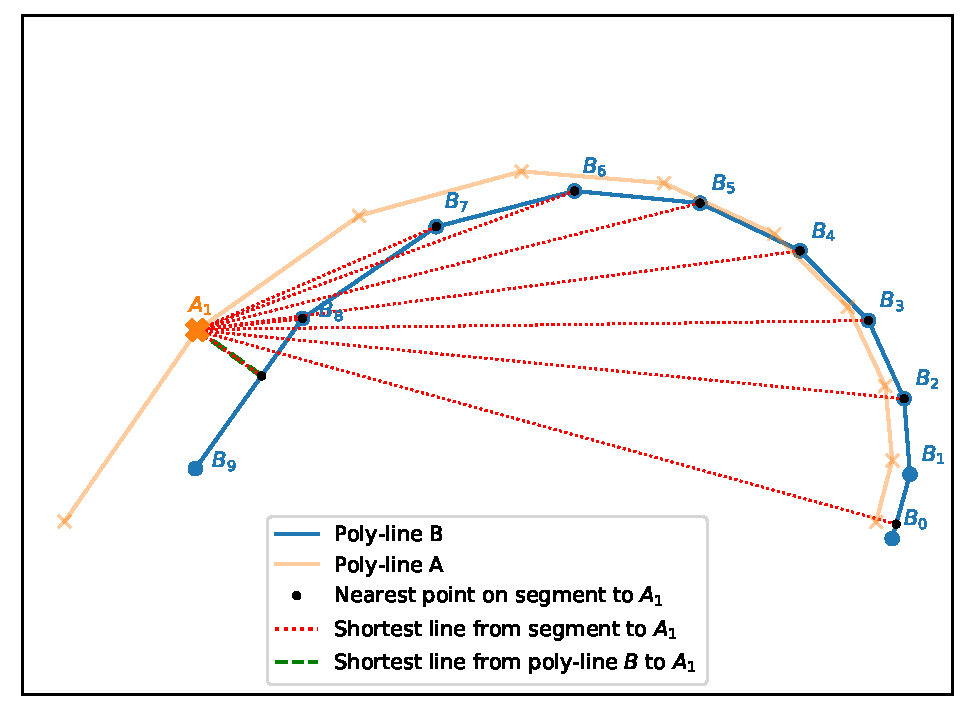
\includegraphics[width=8cm]{images__appendix/spiral_metric_description.pdf}
  \caption{Illustration of the metric used. For each point in line $A$, the shortest distance to each segment in line $B$ is calculated (shown as dotted red lines). The minimum of these distances (corresponding to the line shown in dashed green) is squared.}
  \label{fig:spiral_metric_description}
\end{figure}

First, define a poly-line containing $n$ 2D cartesian coordinates (vertices) as

\begin{equation}
A: \{i \in \mathbb{N};\;i<n\} \longrightarrow \mathbb{R}
^2\end{equation}

We also define a function, $t$, which calculates how far a point $\vec{p}$ is along the line between two other points ($\vec{v}$ and $\vec{w}$):

\begin{equation}
t(\vec{p},\,\vec{v},\,\vec{w}) \equiv \frac{(\vec{p} - \vec{v})\cdot(\vec{v} - \vec{w})}{|\vec{w} - \vec{v}|^2}.
\end{equation}

The minimum distance from $\vec{p}$ to the line segment between $\vec{v}$ and $\vec{w}$ is given by

\begin{equation}
d(\vec{p},\,\vec{v},\,\vec{w}) = \|\left(\vec{v} + \mathrm{min}(\mathrm{max}(t(\vec{p},\,\vec{v},\,\vec{w}),\, 0),\, 1)\;(\vec{w} - \vec{v})\right) - \vec{p}\|
\end{equation}

We then define a ``squared distance'' from the poly-line $A$ (containing $n$ vertices) to the poly-line $B$ (containing $m$ vertices):

\begin{equation}
D(A,\,B) \equiv \frac{1}{n}\sum_{i = 0}^{n} \mathrm{min}\{j \in \mathbb{N}_0,\, j < m;\; d(A_i,\, B_j,\, B_{j+1})^2\}.
\end{equation}

The choice to square the distances and penalize large deviations from other lines was a data-driven choice to improve the results of clustering.

Finally, we define our separation measure between two drawn poly-lines as

\begin{equation}
distance(A,\,B) \equiv D(A,\,B) + D(B,\,A).
\end{equation}


\section{Stacking of multiple SDSS Frames}
\label{appendix:frame_stacking}

 All data required for sigma image creation for stacked frames came from the corrected frames, as detailed in the frame datamodel\footnote{\url{https://data.sdss.org/datamodel/files/BOSS_PHOTOOBJ/frames/RERUN/RUN/CAMCOL/frame.html\#example}}. For each pixel in an SDSS frame, we have

\begin{equation}
\frac{I}{C} = \frac{n}{g} - S + V,
\end{equation}

where $I$ represents the sky-subtracted, corrected image (nanomaggies), $C$ reprents the calibration image, $n$ is the number of electrons captured, $g$ is the gain, $S$ is the Sky value (data units) and $V$ is the dark current, $V = 0 ± \sqrt{v}$ ($v$ being the dark variance).

Given Poisson error,

\begin{equation}
\sigma_n = \sqrt{n}.
\end{equation}

If we stack multiple frames, given $N$ observations of a pixel

\begin{equation}
  \begin{aligned}
n_\mathrm{total} &= \sum_i{n_i} = \sum_i g_i\left(\frac{I_i}{C_i} + S_i - V_i\right),\\
                 &= \sum_{i}\frac{g_i}{C_i}I_i + \sum_i{g_i \left(S_i - V_i\right)} = \sigma_{n_\mathrm{total}}^2.
  \end{aligned}
\end{equation}

This is ideal, and is the level that many fitting software packages work at, we, however, want to return to working in units of nanomaggies on a stacked image, and so further calculation is needed:

\begin{equation}
I = \frac{1}{N}\sum_i I_i,
\end{equation}

\begin{equation}
I = \frac{1}{N}\sum_i C_i\left(\frac{n_i}{g_i} - S_i + V_i\right),
\end{equation}

And so

\begin{equation}
  \sigma_I^2 = \frac{1}{N^2}\sum_i\frac{C_i^2}{g_i^2}\sigma_{n_i}^2 + \frac{1}{N^2}\sum_i C_i^2 \sigma_{S_i}^2 + \frac{1}{N^2}\sum_i C_i^2 \sigma_{V_i}^2.
\end{equation}

We treat the sky value as a constant, such that $\sigma_{S_i}^2 = 0$. Substituting $\sigma_{n_i}^2 = n_i$ as above gives

\begin{equation}
  \sigma_I^2 = \frac{1}{N^2}\sum_i\frac{C_i^2}{g_i^2}n_i + \frac{1}{N^2}\sum_i C_i^2 v_i.
\end{equation}

\begin{equation}
  \sigma_I = \frac{1}{N}\sqrt{\sum_i C_i^2\left(\frac{n_i}{g_i^2} + v_i\right)}.
\end{equation}
Note that this is identical to saying

\begin{equation}
\sigma_I^2 = \frac{1}{N^2}\sum_i\sigma_{I_i}^2.
\end{equation}


\section{Model Fitting}
\label{sec:appendix_model_fitting}
Assume Normal priors on components dictaded by Jaccard clustering ($\mu_x$, $\mu_y$, $q$, $Re$), with the spread given by the spread in the clustered values. We reflect these constraints in the loss function. The gaussian log-likelihood for a value with $\mu$ and $sigma$ is

$$l(\mu, \sigma; x_1, ..., x_n) = -\frac{n}{2}\ln(2\pi) -\frac{n}{2}\ln(\sigma^2) - \frac{1}{2\sigma^2}\sum_{j=1}^n(x_j - \mu)^2$$

We therefore have that our final log-likelihood (to be maximised) for a galaxy with data $D$, uncertainty $S$, parameters $p$ of length $n_p$, with parameter mean $\mu$ and  error $\sigma$, is given by

$$l_{tot}(p) = \sum_{i=0}^{N_x}\sum_{i=0}^{N_x}l(D_{i,j}, S_{i,j}; R_{i,j}(p)\ ) + \sum_{k=0}^{n_p}l(\mu_k, \sigma_{k}; p_k).$$

Alternately,

$$l_{tot}(p) = l\left(0, 1; \frac{D-R(p)}{S}\right) + l(0, 1; \frac{\mu - p}{\sigma}).$$

Where $R(p)$ is the rendering function, which outputs an ($N_x$, $N_y$) image.

The rendering function is the PSF-convolved sum of the separate components, with disc, bulge and bar being variations on the boxy sersic profile:

$$I(\vec{P}) = I_e \exp\left\{-b_n\left[\left(\frac{r\,(\vec{P})}{R_e}\right)^{1/n} - 1\right]\right\}$$

where

$$r\,(\vec{P}) = \left|\begin{pmatrix}
\frac{1}{q} & 0 \\\\
0 & 1
\end{pmatrix}\begin{pmatrix}
\cos\psi & -\sin\psi\\\\
\sin\psi & \cos\psi
\end{pmatrix}\left(\vec\mu - \vec{P}\right)\right|_{\ c}.$$

A disc has $n=1; c=2$, a bulge has $n\in(0.5, 6); c=2$ and a bar has $n\in(0.5, 6); c\in(0.5, 6)$.

To slightly complicate matters, the Sérsic components are rendered at 5x the image resolution, and downsampled using the mean pixel brightness. This is a widely used method of approximating the true pixel value, which is an integration over the area of sky inside the pixel. I.e. for a pixel of size $(\delta_x, \delta_y)$

$$
I_\mathrm{pix}(\vec{P}) = \frac{1}{\delta_x \delta_y}\int_{-\delta_y/2}^{\delta_y/2}\int_{-\delta_x/2}^{\delta_x/2}\mathrm{d}x\mathrm{d}y\ I\left(\vec{P} + \begin{pmatrix}
\delta_x \\\\
\delta_y \\\\
\end{pmatrix}\right).
$$

A logarithmic spiral arm in Galaxy Builder is defined by a brightness $I_s$, spread $s$, minimum and maximum $\theta$ ($a$ and $b$), an amplitude $A$, pitch angle $\phi$, position $\vec\mu$, position angle $\psi$ and axis ratio $q$, where $\vec\mu$, $\psi$ and $q$ are inherited from the disc component. It is multiplied by the disc component to capture the correct exponential falloff with the disc.

$$S(\vec{P}) = I_\mathrm{Disc}(\vec{P}) \times I_s\exp\left(-\frac{1}{s}\min_{\theta\in[a, b]}\left|\left|\vec{P} - \vec\mu - Ae^{\theta\tan\phi}\begin{pmatrix}
\cos\psi & \sin\psi\\\\
-\sin\psi & \cos\psi
\end{pmatrix}
\begin{pmatrix}
q\cos\theta \\\\
\sin\theta \\\\
\end{pmatrix}
\right|\right|^{\ 2}\right)$$


Therefore, for a galaxy with a disc, bulge, bar and $N_s$ spiral arms, we have:

$$R(\vec{P}) = \mathrm{conv}\left(I(\vec{P}; \mathrm{disc}) + I(\vec{P}; \mathrm{bulge}) + I(\vec{P}; \mathrm{bar}) + \sum_{i=0}^{N_s} S(\vec{P}; \mathrm{spiral}_i),\ \mathrm{PSF}\right).$$

We parametrize disc $I_e$ as total Luminosity, given by

$$L_\mathrm{tot} = I_eR_e^2\ 2\pi n\frac{e^{b_n}}{(b_n)^{2n}}\Gamma(2n).$$

Bulge (bar) $I_e$ is reparametrized as ''bulge (bar) fraction``, which we define as

$$F_\mathrm{bulge} = \frac{L_\mathrm{bulge}}{L_\mathrm{disc} + L_\mathrm{bulge}},$$

And is limited to be between 0 and 1. Disc luminosity is allowed to take any value greater than or equal to zero.

Similarly, bulge and bar effective radius are reparametrized as their scale relative to the disc ($R_e = R_e / R_{e,\,\mathrm{disc}}$). Bulge and bar are also restricted to have the same $\mu$.


\section{Ancillary Tables}
\begin{table*}
  \centering
  \caption{The maximum, minimum and default values for model parameters. Note that some parameters were allowed to overflow when fitting, for instance an axis ratio greater 1 (signifying a swap of major and minor axis) was allowed, and corrected for once fitting reached completion. This helped avoid the optimizer encountering parameter bounds and failing to converge. Component roll was similarly unconstrained.}
  \begin{tabular}{l|l|r|r|r|r|r}
\hline
Component & Parameter  & Tuning Minimum & Tuning Maximum \\
          &            &  Bound         & Bound          \\
\hline
disc      & $\mu_x$    & -inf           & inf            \\
          & $\mu_y$    & -inf           & inf            \\
          & roll       & -inf           & inf            \\
          & $q$        & 0.01           & 100            \\
          & $R_e$      & 0              & inf            \\
          & $\Sigma_e$ & 0              & inf            \\
bulge     & $\mu_x$    & -inf           & inf            \\
          & $\mu_y$    & -inf           & inf            \\
          & roll       & -inf           & inf            \\
          & $q$        & 0.01           & 100            \\
          & $R_e$      & 0              & inf            \\
          & $\Sigma_e$ & 0              & inf            \\
          & $n$        & 0.1            & 10             \\
bar       & $\mu_x$    & -inf           & inf            \\
          & $\mu_y$    & -inf           & inf            \\
          & roll       & -inf           & inf            \\
          & $q$        & 0.01           & 100            \\
          & $R_e$      & 0              & inf            \\
          & $\Sigma_e$ & 0              & inf            \\
          & $n$        & 0.1            & 10             \\
          & $c$        & 0.01           & 10             \\
spiral    & $\Sigma_e$ & 0              & inf            \\
          & spread     & 0              & inf            \\
          & falloff    & 0.01           & inf            \\
\hline
  \centering
  \end{tabular}
  \label{table:bad_values}
\end{table*}

\begin{table*}
  \centering
  \caption{Pivot table of reported errors on parameters for our sample of 297 galaxies. Errors quoted are absolute errors.}
  \begin{tabular}{l|l|rrrrrrrr}
  \hline
  component & parameter &  count &  mean &   std &   min &   25\% &   50\% &   75\% &    max \\
  \hline
  disk  & $\Sigma_e$ (nmgy) &    291 &  0.20 &  0.21 &  0.01 &  0.07 &  0.14 &  0.25 &  1.22 \\
        & $r_e$ &    291 &  0.65 &  0.32 &  0.08 &  0.42 &  0.60 &  0.85 &  1.82 \\
        & $\mu_x$ (arcseconds) &    291 &  0.43 &  0.28 &  0.05 &  0.24 &  0.38 &  0.56 &  2.56 \\
        & $\mu_y$ (arcseconds) &    291 &  0.44 &  0.26 &  0.11 &  0.26 &  0.36 &  0.54 &  1.93 \\
        & $b/a$ &    291 &  0.09 &  0.04 &  0.01 &  0.06 &  0.09 &  0.12 &  0.20 \\
        & $\phi$ (radians) &    291 &  1.63 &  0.36 &  0.21 &  1.43 &  1.58 &  1.77 &  2.93 \\
  bulge & $\Sigma_e$ (nmgy) &    272 &  0.75 &  0.96 &  0.00 &  0.16 &  0.39 &  0.85 &  6.75 \\
        & $r_e$ &    272 &  0.08 &  0.05 &  0.00 &  0.05 &  0.07 &  0.10 &  0.47 \\
        & $\mu_x$ (arcseconds) &    272 &  0.13 &  0.08 &  0.00 &  0.09 &  0.12 &  0.16 &  0.72 \\
        & $\mu_y$ (arcseconds) &    272 &  0.13 &  0.07 &  0.00 &  0.09 &  0.11 &  0.16 &  0.51 \\
        & $n$ &    272 &  1.23 &  0.64 &  0.00 &  0.63 &  1.40 &  1.73 &  2.48 \\
        & $b/a$ &    272 &  0.10 &  0.05 &  0.00 &  0.07 &  0.10 &  0.14 &  0.23 \\
        & $\phi$ (radians) &    272 &  1.56 &  0.57 &  0.00 &  1.28 &  1.57 &  1.86 &  3.47 \\
  bar   & $\Sigma_e$ (nmgy) &     92 &  0.31 &  0.39 &  0.00 &  0.06 &  0.16 &  0.39 &  2.36 \\
        & $r_e$ &     92 &  0.16 &  0.12 &  0.02 &  0.06 &  0.14 &  0.20 &  0.87 \\
        & $c$ &     92 &  0.28 &  0.20 &  0.00 &  0.14 &  0.25 &  0.42 &  0.82 \\
        & $\mu_x$ (arcseconds) &     92 &  0.23 &  0.26 &  0.04 &  0.11 &  0.17 &  0.27 &  2.24 \\
        & $\mu_y$ (arcseconds) &     92 &  0.24 &  0.20 &  0.02 &  0.13 &  0.18 &  0.31 &  1.09 \\
        & $n$ &     92 &  0.37 &  0.30 &  0.00 &  0.08 &  0.30 &  0.66 &  0.88 \\
        & $b/a$ &     92 &  0.09 &  0.04 &  0.01 &  0.06 &  0.08 &  0.11 &  0.23 \\
        & $\phi$ (radians) &     92 &  0.69 &  0.98 &  0.00 &  0.06 &  0.10 &  1.17 &  3.57 \\
  \hline
  \end{tabular}
  \label{table:error_values}
\end{table*}
\end{document}
